\documentclass[10pt,twocolumn]{article}
\usepackage{geometry}
\geometry{verbose,headsep=3cm,tmargin=2.5cm,bmargin=2.5cm,lmargin=2.0cm,rmargin=2.0cm}
\usepackage{graphicx}
\usepackage{xcolor}
\usepackage[font=small]{caption}
\usepackage{amsmath,amssymb,latexsym}
\usepackage{marvosym}
\usepackage{url}
\usepackage{lipsum}
\usepackage{bm}
\usepackage{float}
\usepackage[english]{babel}
\usepackage{caption}
%\usepackage{subfigure}
\usepackage{subcaption}
\usepackage{subfloat}
\usepackage{hyperref}
\usepackage{epsf}
\usepackage{float}
\usepackage{mathpazo}
\usepackage{pifont}
\usepackage{graphicx}
%\usepackage{subfig}
\usepackage{wrapfig}
\usepackage{multicol}
\usepackage{enumitem}
\usepackage{xcolor}
\usepackage{framed}
\usepackage[utf8]{inputenc}
% Document font:
\usepackage{charter}
\graphicspath{{DWGs/}}
\newcommand*{\addheight}[2][.5ex]{%
  \raisebox{0pt}[\dimexpr\height+(#1)\relax]{#2}%
}

\begin{document}

\twocolumn[{
\begin{@twocolumnfalse}

  \begin{center}
%\textcolor{lgray}
    \vskip-5em

    \hfill
    \fontsize{10}{10}\selectfont {\textit{Bruxelles, June 2019}}

    \vskip2ex
    
	\vspace{5ex}
	
    \fontsize{24}{10}\selectfont {Least squares regression}
    
    \fontsize{18}{10}\selectfont {a short story on overdetermined linear systems and Moore-Penrose pseudoinverse}

  \noindent%
    
\vskip1ex

{\rule{\textwidth}{0.5pt}}

  \end{center}
  
    \fontsize{7}{10}\selectfont {This work is licensed under the Creative Commons Attribution-NonCommercial-ShareAlike 4.0 International (CC BY-NC-SA 4.0) license.}

\vspace{6mm}

\end{@twocolumnfalse}
}]

\setlength{\parindent}{0cm}

\vspace{10mm}

\setlength{\parindent}{0cm}

\fontsize{14}{10}\selectfont {Kamila Zdybał}

\vspace{2mm}

\fontsize{8}{10}\selectfont {\textit{Université libre de Bruxelles, kamila.zdybal@ulb.ac.be}}

\fontsize{8}{10}\selectfont {\textit{camillejr.github.io/science-docs, kamila.zdybal@gmail.com}}

\vspace{2mm}



\section*{Preface}

Imagine a linear system of equations with more number equations than the number of unknowns.

\,\,

Goal of this paper: explain why Moore-Penrose inverse give a least squares regression.
\,\,

This document is still in preparation. Please feel free to contact me with any suggestions, corrections or comments.

\section*{Keywords}

\textit{overdetermined linear systems, partial least squares regression, Moore-Penrose inverse}

\tableofcontents


\section{References on Least Squares}






\section{Least Squares - the story}





\begin{figure}[H]
\centering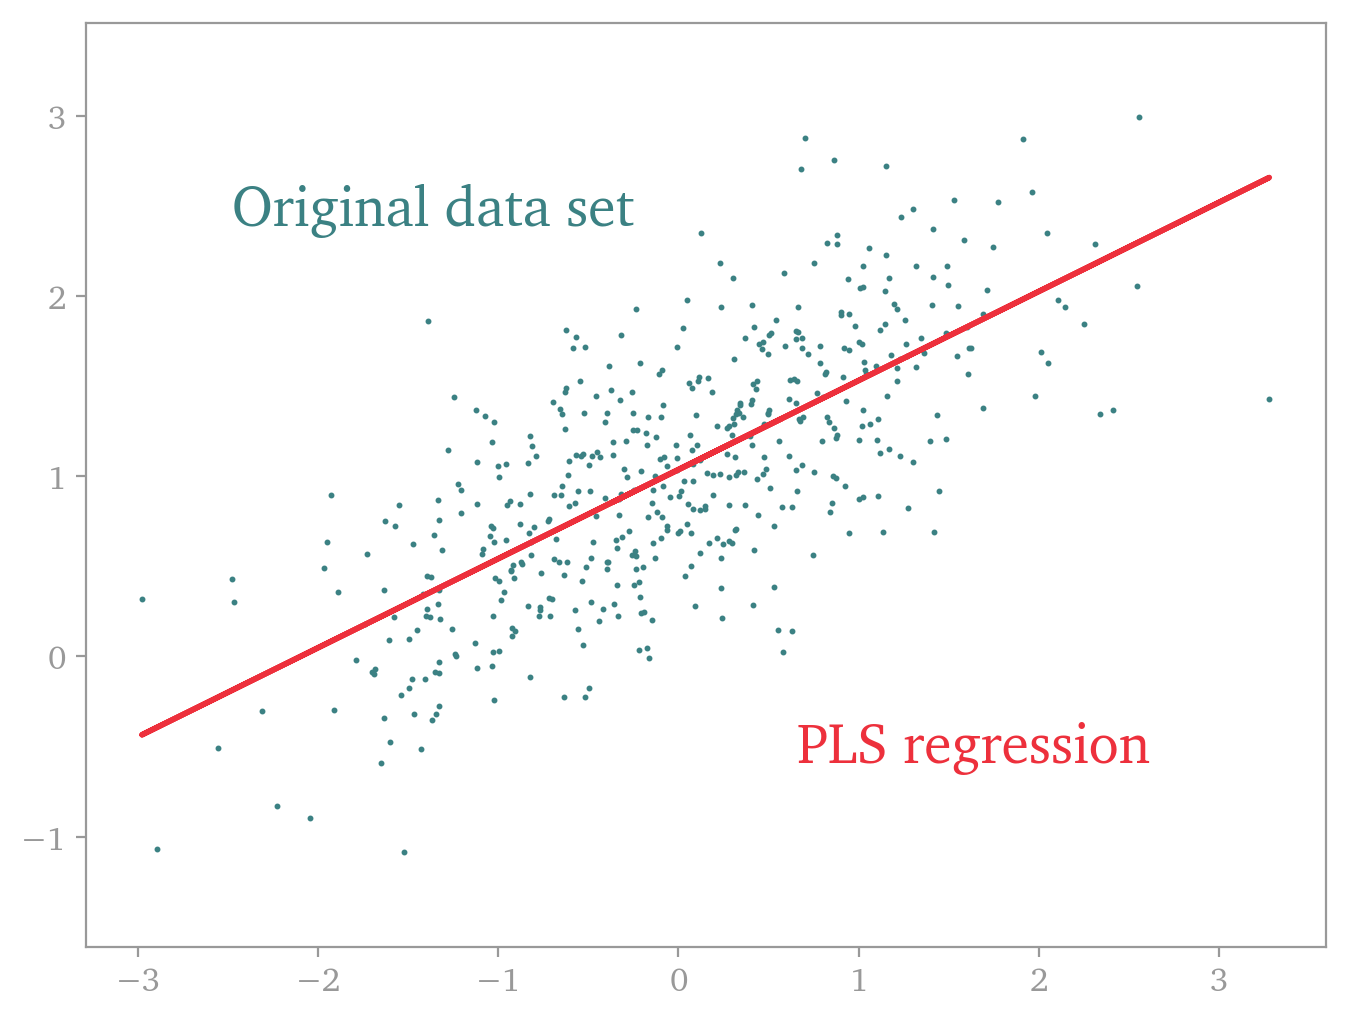
\includegraphics[width=7cm]{linear-regression.png}
\caption{Example of a linear regression.}
\label{fig:linear-regression-demo}
\end{figure}




\section{Partial Least Squares (PLS) regression}

The most general linear equation is of the form:

\begin{equation} \label{eq:linear-equation}
\bm{X} \bm{w} = \bm{y}
\end{equation}

At this point, I ought to give a small justification. In many literature references such as \cite{Strang}, the above equation can be encountered written as $A \vec{x} = \vec{b}$ (with unknown $\vec{x}$) or $\bm{A} \bm{x} = \bm{y}$ (with unknown $\bm{x}$). I decided to write it in a different notation, with the unknown vector $\bm{w}$, since I wanted to highlight the link of algebra with geometry.

To avoid naming confusion, in eq.(\ref{eq:linear-equation}), $\bm{X}$ and $\bm{y}$ contain the actual $x$ and $y$ coordinates of the data points on the $x$ and $y$ axis respectively. Thus, $\bm{X}$ and $\bm{y}$ are known; the vector of unknown coefficients is $\bm{w}$.

This actually follows the notation presented in \cite{Bishop} in Chapter 3 on \textit{Linear Models for Regression}.

2D data example

Have a data set in pairs: (X, Y). X is a vector of N points and Y is a vector of corresponding N points. Together they make a cloud of points on a 2D-plane.

We now say that: X A = Y.

We are interested in finding the coefficients: y = C x + D.












\begin{figure}[H]
\centering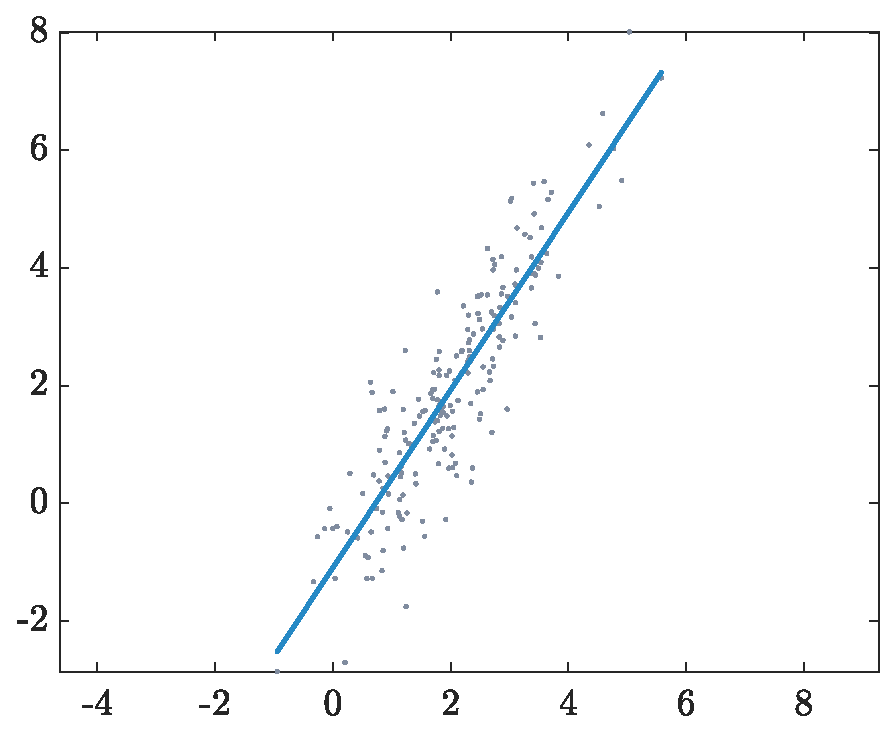
\includegraphics[width=7cm]{LS-linear-basis-functions.eps}
\caption{Linear basis function LS regression.}
\label{fig:LS-linear-basis}
\end{figure}

\begin{figure}[H]
\centering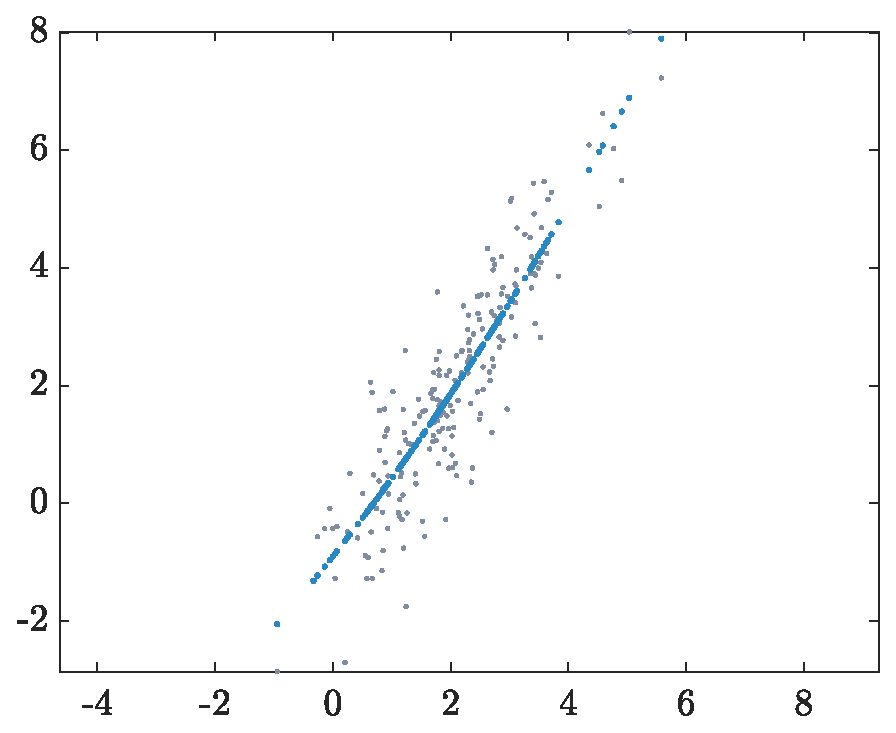
\includegraphics[width=7cm]{LS-nonlinear-basis-functions.eps}
\caption{Non-linear (quadratic) basis function LS regression.}
\label{fig:LS-linear-basis}
\end{figure}











\newpage


\thebibliography{}



\bibitem{Strang} Gilbert Strang, \textit{Introduction to Linear Algebra}, Fifth Edition, 2016

\bibitem{Bishop} Christopher M. Bishop, \textit{Pattern Recognition and Machine Learning}, 2006

\bibitem{Kutz} Nathan Kutz, \textit{Data Driven Discovery of Dynamical Systems and PDEs}, an online lecture 

\bibitem{Tibishrani} T. Hastie, R. Tibshirani, J. Friedman, \textit{Elements of Statistical Learning, Data Mining, Inference, and Prediction}, Second Edition, 2008

 \label{bib:pope}


\end{document}
